
\chapter{Resultados}

\section{Determinaci\'on de la cantidad de prote\'inas.}

La curva de calibraci\'on obtenida por el m\'etodo de \cite{bradford1976rapid} (Fig. \ref{bsa}) es la de una ecuaci\'on de regresi\'on lineal. El valor del coeficiente $R^2$ muy cercano a 1 refleja un buen ajuste lineal de los datos. Los valores de concentraci\'on de prote\'inas se especifican para cada uno de los extractos.

\begin{figure}[hbtp]
	\centering
	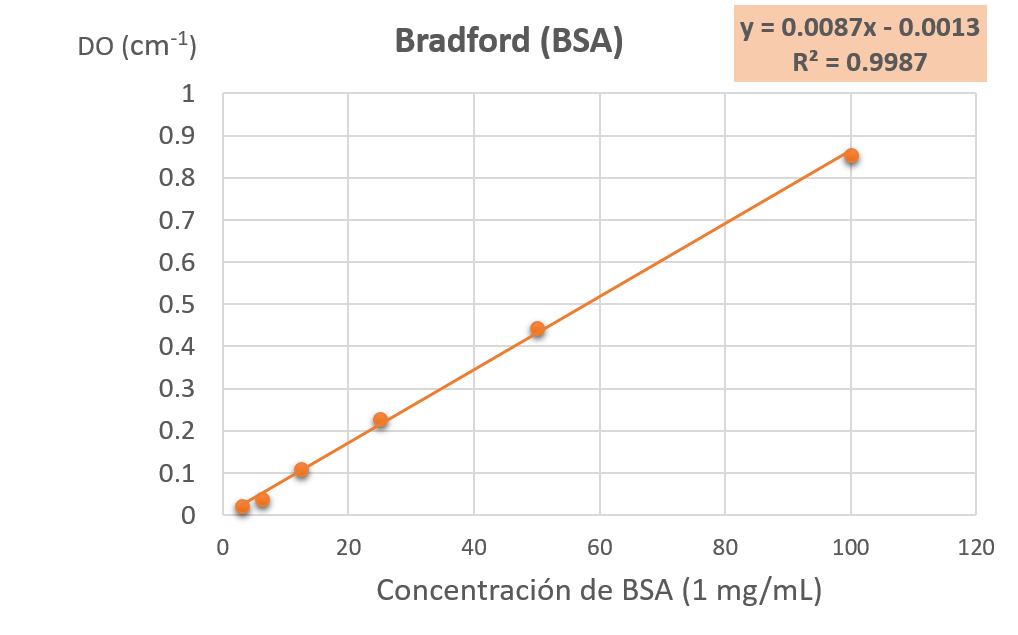
\includegraphics[scale=0.80]{Imagenes/BSA}
	\caption{Representaci\'on de DO obtenida por el reactivo Bradford y la concentraci\'on de Alb\'umina de Suero Bovino.}
	\label{bsa}
\end{figure}

\section{Enzima Super\'oxido Dismutasa (SOD).}

La actividad de la enzima SOD, para los diferentes tratamientos, se determin\'o en plantas no sometidas a estr\'es salino (primer dise\~no experimental). 

\subsection{Actividad enzim\'atica de SOD en extractos obtenidos mediante protocolo de extracci\'on enzim\'atica propuesto por \cite{liu2010exogenous}, con modificaciones.}

La concentraci\'on de prote\'inas de los extractos obtenidos para cada uno de los tratamientos en el caso de la enzima SOD, se muestra en la tabla \ref{cprot}. El ANOVA simple indic\'o que las diferencias entre estos valores no fueron significativas ($F=0.1249$, $p=0.9427$).\\

\begin{table}[h]
	\caption{Concentraci\'on de prote\'ina en $20 \;\mu L$ de las muestras con los diferentes tratamientos: control negativo (C-), etanol (EtOH), DI-31 y \'acido salic\'ilico (AS).}
	\label{cprot}
	\begin{center}
		\begin{tabular}{|c|M{25mm}|M{25mm}|M{25mm}|M{25mm}|c|}
			\hline 
			\textbf{} & \textbf{C-} & \textbf{EtOH} & \textbf{DI-31} & \textbf{AS} \\ 
			\hline 
			$24 \; horas$ &  $12.91 \;\mu g/mL$ & $10.95\; \mu g/mL$  & $10.38\; \mu g/mL$ & $15.55\; \mu g/mL$ \\ 
			\hline 
			$48 \; horas$ &  $8.54 \;\mu g/mL$ & $9.57\; \mu g/mL$  & $14.29 \;\mu g/mL$ & $9.0\; \mu g/mL$ \\ 
			\hline 
			$96 \; horas$ &  $6.87\; \mu g/mL$ & $8.08\; \mu g/mL$  & $7.96\; \mu g/mL$ & $6.36\; \mu g/mL$ \\
			\hline 			
		\end{tabular} 
	\end{center}
\end{table}

\normalsize

En la determinaci\'on de actividad enzim\'atica de SOD con este protocolo, para cada uno de los extractos se analizaron concentraciones diferentes de Pyrogallol ($6.4\;mM$; $3.2\;mM$; $1.6\;mM$ y $0.8\;mM$). \\

Los resultados de velocidad de autoxidaci\'on del Pyrogallol obtenidos para cada uno de los tiempos (24, 48 y 96 horas) se muestran en las tablas \ref{24hSOD}, \ref{48hSOD} y \ref{96hSOD} respectivamente. Los valores de autoxidaci\'on son todos cercanos a cero, no se detect\'o actividad enzim\'atica. \\

Este ensayo se realiz\'o en otras dos especies de plantas, \textit{Nicotiana tabacum} (tabaco) y \textit{Solanum lycopersicum} (tomate) y con diferentes concentraciones de EDTA.  En todos los casos, los resultados obtenidos (no mostrados) fueron similares.\\

\begin{table}[h]
	\caption{Resultados de $\Delta$DO para SOD a las 24 horas de aplicados los tratamientos.}
	\label{24hSOD}
	\begin{center}
		\begin{tabular}{|c|M{25mm}|M{25mm}|M{25mm}|M{25mm}|M{25mm}|c|}
			\hline 
			\textbf{[sustrato]} & \textbf{$\Delta$DO blanco} & \textbf{$\Delta$DO C-} & \textbf{$\Delta$DO EtOH} & \textbf{$\Delta$DO DI-31} & \textbf{$\Delta$DO AS} \\ 
			\hline 
			$6.4mM$ &  $0.001$ & $0.0012$  & $0.0011$ & $0.001$ & $0.001$ \\ 
			\hline 
			$3.2mM$ &  $0.0006$ & $0.0007$  & $0.0006$ & $0.0006$ & $0.0006$ \\ 
			\hline 
			$1.6mM$ &  $0.0003$ & $0.0003$  & $0.0003$ & $0.0003$ & $0.0003$ \\
			\hline 
			$0.8mM$ &  $0.0001$ & $0.0001$  & $0.0001$ & $0.0001$ & $0.0001$ \\
			\hline
		\end{tabular} 
	\end{center}
\end{table}

\normalsize

\begin{table}[h]
	\caption{Resultados de $\Delta$DO para SOD a las 48 horas de aplicados los tratamientos.}
	\label{48hSOD}
	\begin{center}
		\begin{tabular}{|c|M{25mm}|M{25mm}|M{25mm}|M{25mm}|M{25mm}|c|}
			\hline 
			\textbf{[sustrato]} & \textbf{$\Delta$DO blanco} & \textbf{$\Delta$DO C-} & \textbf{$\Delta$DO EtOH} & \textbf{$\Delta$DO DI-31} & \textbf{$\Delta$DO AS} \\ 
			\hline 
			$6.4mM$ &  $0.0005$ & $0.0007$  & $0.0006$ & $0.0007$ & $0.0006$ \\ 
			\hline 
			$3.2mM$ &  $0.0003$ & $0.0004$  & $0.0004$ & $0.0003$ & $0.0004$ \\ 
			\hline 
			$1.6mM$ &  $0.0001$ & $0.0002$  & $0.0002$ & $0.0001$ & $0.0002$ \\
			\hline 
			$0.8mM$ &  $0.00005$ & $0.00005$  & $0.00005$ & $0.00005$ & $0.00005$ \\
			\hline
		\end{tabular} 
	\end{center}
\end{table}

\normalsize


\begin{table}[h]
	\caption{Resultados de $\Delta$DO para SOD a las 96 horas de aplicados los tratamientos.}
	\label{96hSOD}
	\begin{center}
		\begin{tabular}{|c|M{25mm}|M{25mm}|M{25mm}|M{25mm}|M{25mm}|c|}
			\hline 
			\textbf{[sustrato]} & \textbf{$\Delta$DO blanco} & \textbf{$\Delta$DO C-} & \textbf{$\Delta$DO EtOH} & \textbf{$\Delta$DO DI-31} & \textbf{$\Delta$DO AS} \\ 
			\hline 
			$6.4mM$ &  $0.0009$ & $0.001$  & $0.001$ & $0.0011$ & $0.001$ \\ 
			\hline 
			$3.2mM$ &  $0.0005$ & $0.0005$  & $0.0005$ & $0.0005$ & $0.0005$ \\ 
			\hline 
			$1.6mM$ &  $0.0002$ & $0.0002$  & $0.0002$ & $0.0002$ & $0.0002$ \\
			\hline 
			$0.8mM$ &  $0.00007$ & $0.00009$  & $0.0001$ & $0.00004$ & $0.0001$ \\
			\hline
		\end{tabular} 
	\end{center}
\end{table} 

\normalsize

\pagebreak

\subsection{Actividad enzim\'atica de SOD en extractos obtenidos mediante protocolo de extracci\'on enzim\'atica propuesto por \cite{baquero2005catalase}, con modificaciones.}

El extracto enzim\'atico obtenido mediante la segunda metodolog\'ia de extracci\'on conten\'ia $1.64\;\mu g/mL$ de prote\'ina, aproximadamente seis veces menor que la concentraci\'on de prote\'inas presente en los extractos obtenidos mediante el protocolo de extracci\'on de \cite{liu2010exogenous}.\\

En la tabla \ref{AE} se muestra el c\'alculo de la actividad enzim\'atica de SOD a las 24 horas de aplicados los tratamientos, para diferentes concentraciones de Pyrogallol ($10\;mM$; $6.4\;mM$; $3.2\;mM$ y $1.6\;mM$). Se utilizan los valores de Factor de diluci\'on 1 = 30 (Ecuaci\'on \ref{fd1}) y el FD=30 (Ecuaci\'on \ref{FD}).\\

\begin{table}[h]
	\caption{C\'alculo de la actividad enzim\'atica de SOD. El hiperv\'inculo indicado entre par\'entesis conduce a la ecuaci\'on utilizada para el c\'alculo del par\'ametro.}
	\label{AE}
	\begin{center}
		\begin{tabular}{|c|M{14mm}|M{14mm}|M{14mm}|M{14mm}|c|}
			\hline 
			\textbf{} & \textbf{10mM} & \textbf{6.4mM} & \textbf{3.2mM} & \textbf{1.6mM} \\ 
			\hline 
			$Tasa \; de \; autoxidaci\acute{o}n \; del \; Pyrogallol \; (min^{-1})  \; (\ref{tasapyr})$ &  $0.066$ & $0.034$  & $0.028$ & $0.012$ \\ 
			\hline 
			$Tasa \; de \; SOD \; (min^{-1})  \; (\ref{tasasod})$ &  $0.061$ & $0.028$  & $0.025$ & $0.011$ \\ 
			\hline 
			$Inhibici\acute{o}n \; (I) \; (min^{-1})  \; (\ref{inh})$ &  $0.005$ & $0.006$  & $0.003$ & $0.001$ \\
			\hline		
			$\% Inhibici\acute{o}n \; (\%) \; (\ref{inhporc})$ &  $7.614$ & $17.647$  & $10.144$ & $8.333$ \\ 	
			\hline 
			$50\% \; de \; Inhibici\acute{o}n \; (\%) \; (\ref{50inh})$ &  $0.152$ & $0.353$  & $0.203$ & $0.167$ \\ 	
			\hline 
			$Actividad \; de \; SOD \; (unidades \; mg^{-1} \; MF) \; (\ref{act})$ &  $9.137$ & $21.176$  & $12.173$ & $10$ \\ 	
			\hline 
		\end{tabular} 
	\end{center}
\end{table}

\normalsize

Con los resultados de actividad enzim\'atica de SOD para las diferentes concentraciones de Pyrogallol mostradas en la tabla \ref{AE} se obtuvo la curva de cin\'etica enzim\'atica Michaelis-Menten que se muestra en la figura \ref{SODacet}. 

\begin{figure}[hbtp]
	\centering
	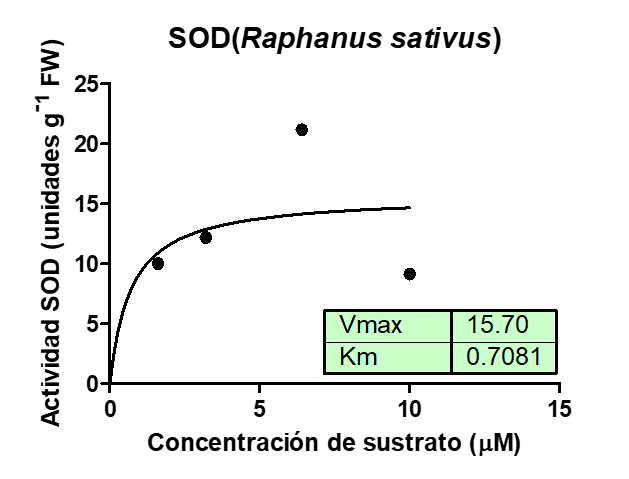
\includegraphics[scale=0.99]{Imagenes/SODacet}
	\caption{Cin\'etica enzim\'atica de Michaelis-Menten de la enzima SOD obtenida mediante el programa \textit{GraphPad Prism}. Se muestran los valores $K_ma$ y $V_{max}$ de SOD en plantas de \textit{R. sativus} que germinaron a partir de semillas que no fueron impregnadas previamente y no estaban sometidas a estr\'es. Se utiliz\'o el protocolo de extracci\'on con acetona \citep{baquero2005catalase}. Se analiza un único caso representativo (n=1) por lo que no se puede realizar análisis estadístico.}
	\label{SODacet}
\end{figure}

\pagebreak

\section{Enzima Catalasa (CAT).}

El extracto enzim\'atico fue preparado a partir de plantas que no estaban sometidas a estr\'es salino utilizando el protocolo de extracci\'on de \cite{liu2010exogenous} (primer dise\~no experimental, ep\'igrafe \ref{d1}). La concentraci\'on de prote\'inas fue de $10.82 \; \mu g/ \mu L$. Con los valores obtenidos se construy\'o la curva de cin\'etica enzim\'atica que se muestra en la figura \ref{cat}.\\

\begin{figure}[hbtp]
	\centering
	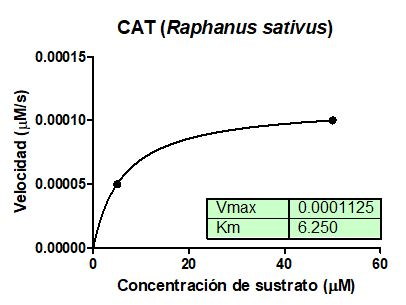
\includegraphics[scale=0.95]{Imagenes/CAT}
	\caption{Cin\'etica enzim\'atica Michaelis-Menten de la enzima CAT obtenida mediante el programa \textit{GraphPad Prism}. Se muestran los valores de $K_ma$ y $V_{max}$ de CAT en plantas de \textit{R. sativus} que germinaron a partir de semillas que no fueron impregnadas previamente y no estaban sometidas a estr\'es. La prote\'ina se extrajo mediante el protocolo de \cite{liu2010exogenous}. Se analiza un único caso representativo (n=1) por lo que no se puede realizar análisis estadístico.}
	\label{cat}
\end{figure}

\section{Enzima Polifenol Oxidasa (PPO).}\

Los extractos obtenidos mediante el segundo protocolo de extracci\'on enzim\'atica \citep{baquero2005catalase}, no mostraron resultados de la enzima PPO, no hubo variaci\'on en la DO, ni en la pendiente. 

\pagebreak

\subsection {PPO, primer dise\~no experimental: plantas no sometidas a estr\'es salino.}

El extracto enzim\'atico de plantas no sometidas a estr\'es salino, obtenido mediante el protocolo de extracci\'on propuesto por \cite{liu2010exogenous} (ep\'igrafe \ref{p1}), present\'o una concentraci\'on de $10.26 \;\mu g/ \mu L$ de prote\'ina. En la figura \ref{POd1} se muestra la cin\'etica enzim\'atica de Michaelis-Menten obtenida para las concentraciones de L-DOPA: $10\;mM$; $5\;mM$; $2.5\;mM$ y $1.125\;mM$.\\

\begin{figure}[hbtp]
	\centering
	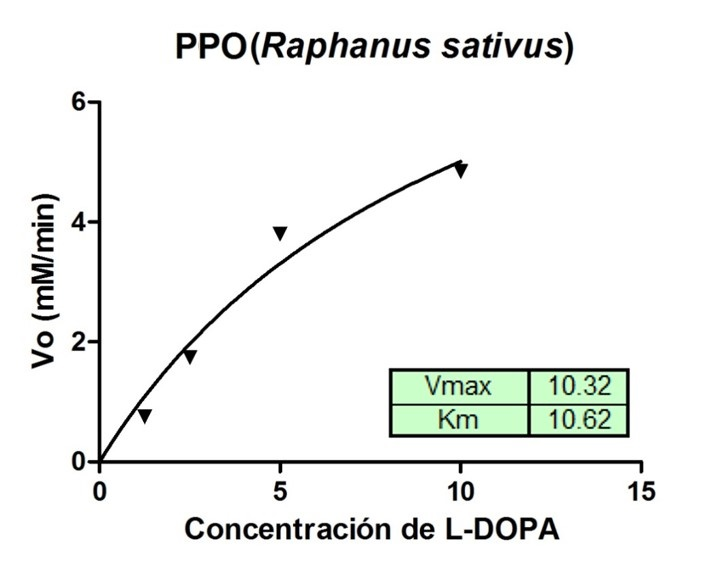
\includegraphics[scale=0.9]{Imagenes/POd1}
	\caption{Cin\'etica enzim\'atica Michaelis-Menten de la enzima PPO obtenida mediante el programa \textit{GraphPad Prism}. Se muestran los valores de $K_ma$ y $V_{max}$ de PPO en plantas de \textit{R. sativus} que germinaron a partir de semillas que no fueron impregnadas previamente y no estaban sometidas a estr\'es. El extracto se obtuvo mediante el protocolo de extracci\'on de \citep{liu2010exogenous}. Se analiza un único caso representativo (n=1) por lo que no se puede realizar análisis estadístico.}
	\label{POd1}
\end{figure} 

\pagebreak

\subsection {PPO, segundo dise\~no experimental: plantas sometidas a estr\'es salino.}

Seg\'un el procedimiento de \cite{liu2010exogenous}, con modificaciones, se obtuvieron dos extractos de plantas con tratamientos diferentes: control negativo ($10,13 \;\mu g/ \mu L$ de prote\'ina) y planta sometida a estr\'es salino ($9,78 \;\mu g/ \mu L$ de prote\'ina). Se muestra la cin\'etica enzim\'atica de Michaelis-Menten obtenida en la figura \ref{POkmVmax} para las concentraciones de L-DOPA: $7\;mM$; $5\;mM$ y $2.5\;mM$.\\

La comparaci\'on de los valores de $K_ma$ y $V_{max}$ obtenidos en cada uno de los extractos, se muestra en la figura \ref{PObarra}.\\

\medskip
\medskip
\medskip

\begin{figure}[h!!!!]
	\begin{subfigure}{.5\textwidth}
		\centering
		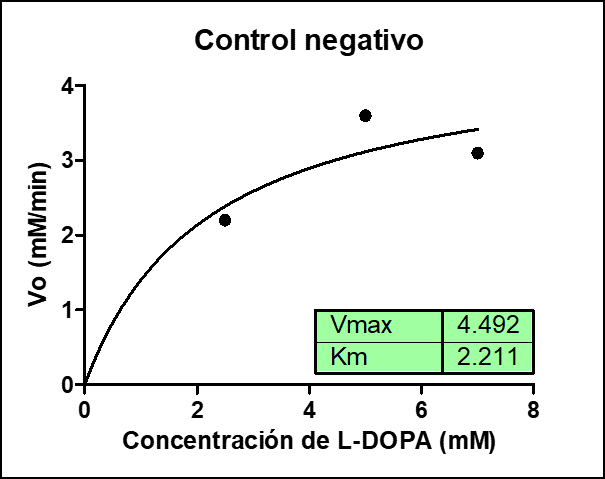
\includegraphics[width=.9\linewidth]{Imagenes/POnada}
		\caption{}
		\label{a}
	\end{subfigure}
	\begin{subfigure}{.5\textwidth}
		\centering
		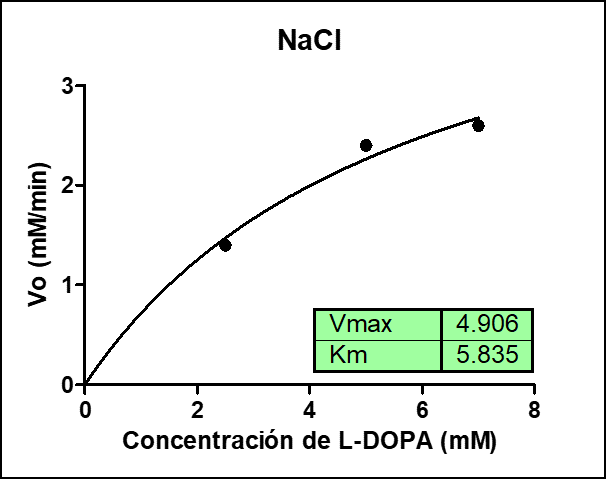
\includegraphics[width=.9\linewidth]{Imagenes/PONaCl}
		\caption{}
		\label{b}
	\end{subfigure}
	\caption{Cin\'etica enzim\'atica Michaelis-Menten de la enzima PPO obtenida mediante el programa \textit{GraphPad Prism}. Se muestran los valores de $K_ma$ y $V_{max}$ de PPO en plantas de \textit{R. sativus} que germinaron a partir de semillas impregnadas previamente con NaCl (sometidas a estr\'es salino) (b) y su control negativo (a). El extracto se obtuvo mediante el protocolo de extracci\'on de \citep{liu2010exogenous}. Se analiza un único caso representativo (n=1) por lo que no se puede realizar análisis estadístico.}
	\label{POkmVmax}
\end{figure}

\pagebreak

\begin{figure}[h!!!!]
	\begin{subfigure}{.5\textwidth}
		\centering
		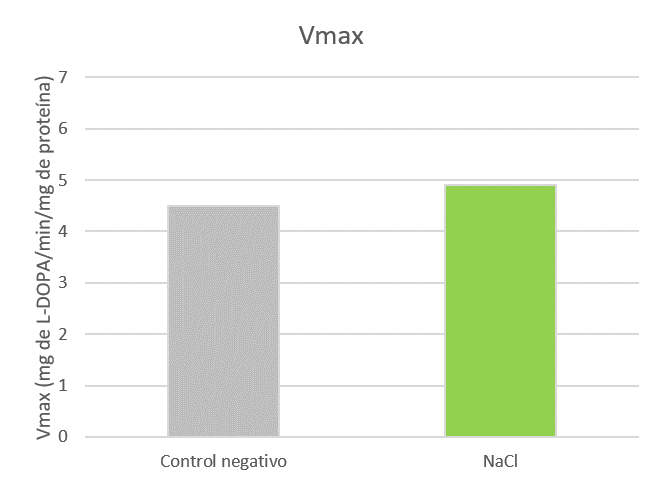
\includegraphics[width=.91\linewidth]{Imagenes/Vmax}
		\caption{}
		\label{1}
	\end{subfigure}
	\begin{subfigure}{.5\textwidth}
		\centering
		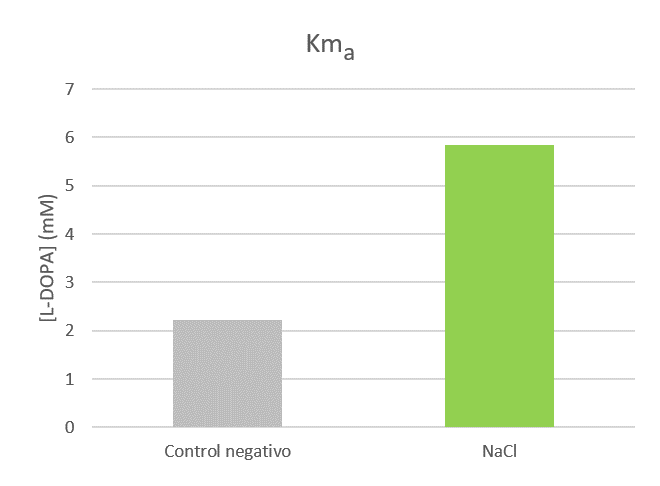
\includegraphics[width=.99\linewidth]{Imagenes/Km}
		\caption{}
		\label{2}
	\end{subfigure}
	\caption{Valores de $V_{max}$ (a) y $K_ma$ (b) de PPO obtenidos en plantas de \textit{R. sativus}, control negativo y sometidas a estr\'es por salinidad.}
	\label{PObarra}
\end{figure}

\medskip
\medskip

Como se observa en la figura \ref{PObarra} los valores de $V_{max}$ de las plantas control son muy similares a los obtenidos para las plantas sometidas a estr\'es por salinidad, pero si se observa un cambio en los valores de $K_ma$.
